 
%%%%%%%%%%%%%%%%%%%%%%%%%%%%%%%% -*-LaTeX-*-%%%%%%%%%%%%%%%%%%%%%%%%%%%%%%%%%%%%%%%%%%%%%%%%%%%
%%% 
%%% standard texheader fo writing extended documents
%%% 
%%% 
%%% 
%%% 
%%% 
%%%%%%%%%%%%%%%%%%%%%%%%%%%%%%%%%%%%%%%%%%%%%%%%%%%%%%%%%%%%%%%%%%%%%%%%%%%%%%%%%%%%%%%%%%%%%%% 

%%%%%%%%%%%%%%%%%%%%%%%%%%%%% **** header *****%%%%%%%%%%%%%%%%%%%%%%%%%%%%%%%%%%%%%%%%%%%
\documentclass[ucs]{beamer}
\mode<presentation>
%%%%%%%%%%%%%%%%%%%%%%%%%%% ### used packages ###%%%%%%%%%%%%%%%%%%%%%%%%%%%%%%%%%%%%%%%%%%%

%%%%%%%%%%%%%%%%%%%%%%%%% # standardmaessig verwendbar #%%%%%%%%%%%%%%%%%%%%%%%%%%%%%%%%%%%%%%%%
% \usepackage[ngerman]{babel}      %% neue deutsche Rechtschreibung
\usepackage[english]{babel}
% \usefonttheme[onlymath]{serif}
% \usepackage[utf8]{inputenc}    
\usepackage{graphicx}            %% include graphics
\usepackage{float}               %% determine image positions
%% \usepackage{soul}             %% offers additional types of text formatil
%% HAS TO BE INSTALLED MANUALLY
%% \usepackage{ellipsis}         %% HAS TO BE INSTALLED MANUALLY
\usepackage{xspace}             
\usepackage{tabularx}             %% tables
\usepackage[font={footnotesize}]{caption}%% description of images and tables 
\usepackage{booktabs}            %% formatting of tables
\usepackage{rotating}            
\usepackage{multirow}
\usepackage{geometry}            %% page geometry 
\usepackage{scrpage2}            %% page layout
\usepackage{dsfont}              %% math font \mathds{R}, => "Real

%% Numbers"  
% \usepackage{mathtools}
% \usepackage[absolute,overlay]{textpos}
% \usepackage{bm}
\usepackage{mathabx}
\usepackage{allrunes}      
% \usepackage{natbib}

\usepackage{amssymb}
% \usepackage{amsthm}
\usepackage{amsmath}
% \usepackage[linkbordercolor={0 0 1}]{hyperref} %% links
% \usepackage[table]{xcolor}
% \PassOptionsToPackage{xcolor}{table}
\usepackage{colortbl}

\usepackage[expansion=false]{microtype} %% for pdfTeX 1.4 or later
\usepackage{comment}
\usepackage{mathtools}
% usepackage{comment}
% \usepackage{wasysym}

% \usepackage{eurosym}

\usepackage{animate}
\usepackage{nicefrac}
\usepackage{algpseudocode}
\usepackage{algorithm}
\usepackage{siunitx}
% \usepackage{wrapfig}
\usepackage{tikz}
\usetikzlibrary{shapes.geometric}
% \usepackage{lmodern}\usepackage{polski}
\usepackage{mhchem}
\usepackage{ogonek}
\usepackage{calc}
% \clearscrheadfoot %% clear all 6 column fields
% \pagestyle{scrheadings} 
% \cfoot[\pagemark]{\pagemark}
% \setheadwidth{text}
% \setheadsepline[text]{0.3mm}
% \ohead{\headmark}
% \automark[chapter]{chapter}
% \renewcommand{\headfont}{\bfseries}

%%%%%%%%%% Crystallographic Symbols %%%%%%%%%%%%%%%%%%%%%%%%%
%%% Needs the font cryst.pfb installed
%%% Symbol is created by \cry{xxx}
\DeclareFontFamily{U}{cry}{\hyphenchar\font=-1}
\DeclareFontShape{U}{cry}{m}{n}{ <-> cryst}{}
\newcommand{\cry}[1]{{\usefont{U}{cry}{m}{n} \symbol{#1}}}

\newenvironment{packed_item}{
  \begin{itemize}
    \setlength{\itemsep}{0pt}
    \setlength{\parskip}{0pt}
    \setlength{\parsep}{0pt}
  }{\end{itemize}}

% \setlength{parindent}{0pt}

\tikzset{
  every overlay node/.style={
    draw=white,fill=white,rounded corners,anchor=north west,
  },
}
% Usage:
% \tikzoverlay at (-1cm,-5cm) {content};
% or
% \tikzoverlay[text width=5cm] at (-1cm,-5cm) {content};
\def\tikzoverlay{%
  \tikz[baseline,overlay]\node[every overlay node]
}%



%%%%%%%%%%%%%%%%%%%%%%%%%%%%%% ### macros ###%%%%%%%%%%%%%%%%%%%%%%%%%%%%%%%%%
\newcommand{\latex}{\LaTeX\xspace}  %% \latex for "LaTeX"
\newcommand{\tex}{\TeX\xspace}      %% \tex for "TeX
\newcommand{\MTFIO}{\textbf{[MTFIO]}}
\newcommand{\euler}{\mathit{e}}
\newcommand{\FT}[1]{\mathcal{F}\left(#1\right)}
\newcommand{\iFT}[1]{\mathcal{F}^{-1}\left(#1\right)}

\newcommand{\overbar}[1]{\mkern 1.5mu\overline{\mkern-1.5mu#1\mkern-1.5mu}\mkern 1.5mu}
\DeclareMathOperator\caret{\raisebox{1ex}{$\scriptstyle\wedge$}}

%%%%%%% style options
\usetheme{PaloAlto}
\begin{comment}
\makeatletter
\setbeamertemplate{sidebar canvas right}{}
\setbeamertemplate{sidebar right}{}
%\setbeamercolor{titlelike}{parent=structure,bg=yellow!15!orange}
\setbeamercolor{logo}{bg=blue!15!black}
\setbeamercolor{logo}{bg=blue!15!black}
\setbeamercolor{frametitle}{bg=blue}     %controls the color of the headline
%\setbeamercolor{sidebar}{bg=blue}

\setbeamertemplate{sidebar}{%
\begin{tikzpicture}[remember picture,overlay]
\shade[top color=gray!85,bottom color=gray!85,middle color=white]
([shift={(0.5cm,-0.5cm)}]current page.north west)
rectangle
([shift={(-0.5cm,0.5cm)}]current page.south east);
\end{tikzpicture}%   
}


\makeatother
\end{comment}
\definecolor{msl}{RGB}{16,16,100}
\usecolortheme[RGB={16,16,100}]{structure}
\setbeamercolor{frametitle}{bg=msl}
\setbeamertemplate{blocks}[rounded][shadow=false]
%\setbeamercolor{sidebar}{bg=msl}
\setbeamercolor{title in sidebar}{fg=white}
\definecolor{logoCol}{RGB}{12,12,84}
\setbeamercolor{logo}{bg=msl}
\setbeamertemplate{title page}[default][colsep=-4bp,rounded=true]


\definecolor{breakColor}{HTML}{7777FF}
\definecolor{lgrey}{HTML}{777777}
\definecolor{myblue}{HTML}{000066}
\definecolor{mypurple}{HTML}{6600CC}
\definecolor{mygreen}{HTML}{005522}
\definecolor{myorange}{HTML}{FF6600}
\definecolor{lgrey}{HTML}{777777}
\definecolor{cellOne}{HTML}{81F7BE}
\definecolor{cellTwo}{HTML}{A9BCF5}
\definecolor{mslGrad}{HTML}{73D7FF}

\colorlet{titleright}{msl!60!mslGrad}
%\colorlet{titlemid}{msl!97!white}
\colorlet{titlecentral}{msl!85!mslGrad}
\colorlet{titleleft}{msl}%!97!mslGrad}

\makeatletter

\pgfdeclarehorizontalshading{beamer@frametitleshade}{\paperheight}{%
  color(\beamer@sidebarwidth)=(titleleft);%
  %  color(8cm)=(titlecentral);%
  color(\paperwidth)=(titleright)%
}

\pgfdeclareverticalshading[titleleft,titleright]{beamer@sidebar}{\beamer@sidebarwidth}{%
  color(0pt)=(titleright);%
  color(\sidebarheight/3)=(titlecentral);%
  color(\sidebarheight)=(titleleft)%
}

\setbeamertemplate{headline}{%
  \begin{beamercolorbox}[wd=\paperwidth]{frametitle}%
    \ifx\beamer@sidebarside\beamer@lefttext%
    \else%
    \hfill%
    \fi%
    \ifdim\beamer@sidebarwidth>0pt%  
    \usebeamercolor[bg]{logo}%
    \begin{pgfpicture}{0pt}{0pt}{\paperwidth}{\beamer@headheight}%
      \usebeamercolor{frametitle right}%
      \pgfpathrectangle{\pgfpointorigin}{\pgfpoint{\paperwidth}{\beamer@headheight}}%
      \pgfusepath{clip}%
      \pgftext[left,base]{\pgfuseshading{beamer@frametitleshade}}%
    \end{pgfpicture}%
    \vskip-\beamer@headheight%
    \vrule width\beamer@sidebarwidth height \beamer@headheight%
    \hskip-\beamer@sidebarwidth%
    \hbox to \beamer@sidebarwidth{\hss\vbox to
      \beamer@headheight{\vss\hbox{\color{fg}\insertlogo}\vss}\hss}%
    \else%
    \vrule width0pt height \beamer@headheight%  
    \fi%
  \end{beamercolorbox}%
}

\setbeamertemplate{sidebar canvas left}{%
  \pgfuseshading{beamer@sidebar}%
}

\makeatother


% \usetheme{Warsaw}
% \usecolortheme{seahorse}
% \usecolortheme{rose}
% \usefonttheme[onlylarge]{structuresmallcapsserif}

%%%%%%%%%%%%%%%%%%%%%%%%%%%% ***** Document *****%%%%%%%%%%%%%%%%%%%%%%%%%%%%%
%%% 
%%% 
%%%%%%%%%%%%%%%%%%%%%%%%%%%%%%%%%%%%%%%%%%%%%%%%%%%%%%%%%%%%%%%%%%%%%%%%%%%%%% 
\title[]{Summary of R functions}
% \subtitle{Master presentation}
%\author[]{Benedikt H\"{a}usele}
\date[2021-07]{2021-07}
%\institute{University of Konstanz}

\begin{document}
  
  \begin{frame}
    \titlepage
  \end{frame}
  
  \section{Basics}
  
  \begin{frame}
    \frametitle{Simple arithmetics}
       \begin{columns}[T]
      \begin{column}{0.5\textwidth}
          \begin{block}{Adding}
        \ttfamily > 17 + 4 \newline [1] 21
           \end{block}
     \begin{block}{Subtraction}
        \ttfamily > 17 - 4 \newline [1] 13
      \end{block}
      \begin{block}{Multiplication}
         \ttfamily > 17 * 4 \newline [1] 61
       \end{block}
           \begin{block}{Exponentiation}
       \ttfamily > 17 $\caret$ 4  \rmfamily ~~or~~ \ttfamily 17 ** 4
       \newline [1] 83521
     \end{block}
   
      \end{column}    
      \begin{column}{0.5\textwidth}
        
      \begin{block}{Division}
        \ttfamily > 17 / 4 \newline [1] 4.25
      \end{block}
      
      
      \begin{block}{Integer Division}
  \ttfamily > 17 \%/\% 4 \newline [1] 4
\end{block}
  \begin{block}{Modulus}
    \ttfamily > 17 \%\% 4 \newline [1] 1
  \end{block}

      \end{column}
    \end{columns}
%    \begin{block}{Reasons for fractionation}
%      \begin{enumerate}
%        \item Isolation of substances
%      \end{enumerate}
 %   \end{block}
  \end{frame}
  
   \begin{frame}
    \frametitle{Assignments, basic functions, local environment}
  \begin{block}{Help}
    \texttt{?$<$function$>$} $\rightarrow$ show help text for function\newline
    Press "Q" in order return to command prompt
  \end{block}
  \begin{block}{Declare and assign an object with value}
    \texttt{ var <- 10 } ( or {\texttt{ 10 -> var }} )
  \end{block}
  \begin{block}{List environment objects}
  \texttt{ls()}
  \end{block}
  \begin{block}{Get information about an object}
  \texttt{str(var)}
  \end{block}
  \begin{block}{Print (to console)}
  \texttt{print("Text")}
    \texttt{print(a)}
  \end{block}
 \end{frame}  

 \begin{frame}
  \frametitle{Numeric functions ("Scalar" / element-wise)}
    \begin{columns}[T]
    \begin{column}{0.5\textwidth}
      \begin{block}{Exponential function}
\texttt{> exp(1)} \newline [1] 2.718282
      \end{block}
  
  \begin{block}{Trigonometric functions }
\footnotesize \ttfamily>\! sin(0) >\! cos(pi) >\! tan(pi/4) \newline
[1] 0 ~  [1] -1 ~~  [1] 1
    \end{block}
    \begin{block}{Absolute values}
\ttfamily > abs(-40) \newline [1] 40
  \end{block}    
  
%  \begin{block}{Hyperbolic functions (I)}
%   x 
%  \end{block}
%  \begin{block}{Hyperbolic functions (II)}
%  x
%  \end{block}
  
    \end{column}
    \begin{column}{0.5\textwidth}
      
        \begin{block}{Square Root}
        \texttt{> sqrt(4)}\newline          [1] 2
      \end{block}

\begin{block}{Logarithms}
\texttt{> log(x) } ~~ natural \newline

\texttt{> log10(x) } ~~ base of 10 \newline

\texttt{> log(x, base) } ~~ variable base \newline
\end{block}


      
    \end{column}
  \end{columns}
\end{frame}


\begin{frame}
        \frametitle{Data structures: \texttt{Vector} generation}
 % \begin{columns}[T]%$   \begin{column}{0.5\textwidth}
    \begin{block}{Combination}
\ttfamily > vec <- c(1.2, 2.3, 4.5, 7, 9, 10)\newline
> print(vec) \newline
[1]  1.2  2.3  4.5  7.0  9.0 10.0
     \end{block}

     \begin{block}{Dot operator (Integer sequence)}
\ttfamily > vec <- 1:5 \newline
> print(vec) \newline
[1] 1 2 3 4 5
     \end{block}
   
     \begin{block}{General sequence}
\ttfamily >  seq(from = 2,  to = 10, by = 2)\newline
[1] 2 4 6 8 10
     \end{block}
   
%   \end{column}
%      \begin{column}{0.5\textwidth}
%      \end{column}
%\end{columns}
  \end{frame}

\begin{frame}
  \frametitle{Data structures: \texttt{Vector} specific functions}
  \begin{block}{Length of a vector}
    \ttfamily
    > vec <- 3:27 \newline
    > length(vec)
    [1] 25
  \end{block}
  
  \begin{block}{Sorting}
    \ttfamily > vec <- c(1, 63, 45, 27, 34)\newline
    > sort(vec)\newline
    [1] 1 27 34 45 63
  \end{block}
  
  \begin{block}{Reversing}
    \ttfamily > vec <- 1:5\newline
    > rev(vec)\newline
    [1] 5 4 3 2 1
  \end{block}
  
  %\begin{block}{Clearing from duplicates}
  %\ttfamily
  %> vec
  %\end{block}
  
\end{frame}

\begin{frame}
  \frametitle{Data structures: \texttt{Vector} }
  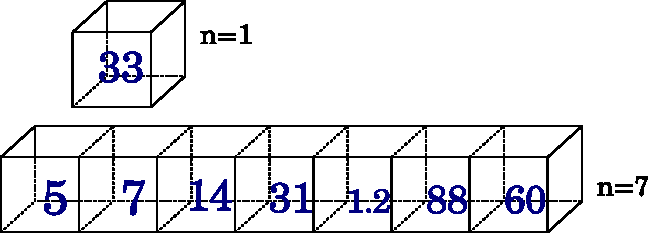
\includegraphics[width=1\linewidth]{./imgs/vector.pdf}
\end{frame}

\begin{frame}
  \frametitle{Data structures: \texttt{Vector} subsetting (I)}
  
  \begin{block}{By single index}
    \ttfamily
    > vec <- seq(from = 10, to 50, by = 0,1)\newline
    > vec[5] \newline
    [1] 
  \end{block}
  
  \begin{block}{By index vector}  
    \ttfamily
    > vec <- seq(from = 10, to 50, by = 0,1)\newline
    > vec[5:10]\newline
    [1] 10.4 10.5 10.6 10.7 10.8
  \end{block}
  
  \begin{block}{All but ...}
    \ttfamily
    > vec <- seq(from = 10, to 50, by = 0,1)\newline
    > vec[-(3:4)] \newline
    [1] 10 10.1 10.4 10.5 10.6
  \end{block}
  
\end{frame}





\begin{frame}
  \frametitle{Descriptive statistical parameters (I)}

  \ttfamily vec <- c(11:30, 15:40)
  \begin{block}{Arithmetic Mean}
    \begin{columns}
      \begin{column}{0.6\textwidth}       
    \ttfamily > mean(vec)
      \end{column}
          \begin{column}{0.4\textwidth}
\[ 
\overbar{x} = \frac{1}{n}\sum_{i=1}^{n}{x_i}
\] 
      \end{column}
  \end{columns}
  \end{block}

\begin{block}{Median}
  \begin{columns}
    \begin{column}{0.5\textwidth}       
      \ttfamily > median(vec)
    \end{column}
    \begin{column}{0.5\textwidth} \[ \tilde{x} =
      \small \begin{cases}
   x_{m+1}  ~~~\, \forall ~n = 2m + 1   \\
   \frac{ x_m + x_{m+1} }{2} ~ \forall~ n = 2m  
%   \emph{$w_{ij}$}, if  -1$\leq$\emph{$w_{ij}$}$\leq$1\\ 
%   -1, if \emph{$w_{ij}$}$<$-1 \\
%   1, if \emph{$w_{ij}$}$>$1 
   \end{cases}   
      \] 
    \end{column}
  \end{columns}
\end{block}
\end{frame}

\begin{frame}
  \frametitle{Descriptive statistical parameters (II)}
\vspace*{-1.75ex}
\begin{block}{Variance of sample}
  \begin{columns}
    \begin{column}{0.55\textwidth}       
\small      \ttfamily > sd(vec)
    \end{column}
  
    \begin{column}{0.45\textwidth}
           \scriptsize
      \[  
s^2 = \frac{1}{n-1} \sum_{i=1}^{n}{(x_i - \overbar{x})^2 } 
      \] 
    \end{column}
  \end{columns}
\end{block}
\vspace*{-1.25ex}
\begin{block}{Variance of population}
  \begin{columns}
    \begin{column}{0.55\textwidth}       
\small      \ttfamily > var(vec) * n / (n-1)
    \end{column}
    \begin{column}{0.45\textwidth}
                            \scriptsize
      \[ 
      \sigma^2 = \frac{1}{n} \sum_{i=1}^{n}{(x_i - \overbar{x})^2 }
%      \overbar{x} = \frac{1}{n}\sum_{i=0}^{n}{x_i}
      \] 
    \end{column}
  \end{columns}
\end{block}
\vspace*{-1.25ex}
\begin{block}{Standard deviation of sample}
  \begin{columns}
    \begin{column}{0.55\textwidth}       
\small      \ttfamily > sd(vec)
    \end{column}
      \begin{column}{0.45\textwidth}
                 \scriptsize
      \[  
      s = \sqrt{\frac{1}{n-1} \sum_{i=1}^{n}{(x_i - \overbar{x})^2 } }
      \] 
    \end{column}
  \end{columns}
\end{block}
\vspace*{-1.25ex}
\begin{block}{Standard deviation of population}
  \begin{columns}
    \begin{column}{0.55\textwidth}             
     \small
      \ttfamily > sd(vec) * sqrt( n / (n-1) )
    \end{column}
    \begin{column}{0.45\textwidth}
                 \scriptsize
      \[ 
\sigma = \sqrt{\frac{1}{n} \sum_{i=1}^{n}{(x_i - \overbar{x})^2 } }
      \] 
    \end{column}
  \end{columns}
\end{block}
\end{frame}


\begin{frame}
  \frametitle{Descriptive statistical parameters (III)}
  \ttfamily
  vec.x <- 11:30\\
  vec.y <- seq( from = 101, to = 139, by = 2 ) \\

  \begin{block}{Covariance of 2 \texttt{Vector}\,s}
    \begin{columns}
      \begin{column}{0.4\textwidth}       
        \ttfamily > cov(vec.x, vec.y)
      \end{column}
        \begin{column}{0.6\textwidth}
      \scriptsize \rmfamily
      \[ 
    \text{Cov}(X,Y) = \frac{1}{n-1} \sum_{i=1}^{n}{\left(x_i - \overbar{x}\right)\left(y_i - \overbar{y}\right)  }
      \] 
    \end{column}
    \end{columns}
  
  \end{block}

\begin{block}{Correlation of 2 \texttt{Vector}\,s}
  \begin{columns}
    \begin{column}{0.4\textwidth}       
      \ttfamily > cor(vec)
    \end{column}
        \begin{column}{0.6\textwidth}
  \scriptsize
  \[ 
  r(X,Y) = \frac{\displaystyle
     \sum_{i=1}^{n}{\left(x_i - \overbar{x}\right)\left(y_i - \overbar{y}\right) }
  }{ \displaystyle
     \sqrt{ \sum_{i=1}^{n}{\left(x_i - \overbar{x}\right)^2}
            \sum_{i=1}^{n}{\left(y_i - \overbar{y}\right)^2}  }
  }
  \] 
\end{column}
\end{columns}
\end{block}


 \end{frame}



\begin{frame}
  \frametitle{Data types: \texttt{Numeric} \& \texttt{Character}}
     
\end{frame}


  \begin{frame}
    \frametitle{Data structures: \texttt{List}}
 %   \frametitle{Why separate things in science?}
  \end{frame}
  
  \begin{frame}
    \frametitle{Data structures: \texttt{Data Frame}}
    %   \frametitle{Why separate things in science?}
  \end{frame}


  
  \begin{frame}
    \frametitle{blank}
    \begin{columns}[T]
      \begin{column}{0.5\textwidth}
      \end{column}
     \begin{column}{0.5\textwidth}
      \end{column}
    \end{columns}
  \end{frame}
  
  
\end{document}
%%% Local Variables:
%%% mode: latex
%%% TeX-master: t
%%% End:
